\let\lesson\undefined
\newcommand{\lesson}{\phantomlesson{Bài 4.}}


\setcounter{section}{2}
\section{Bài tập trắc nghiệm}
\begin{enumerate}[label=\bfseries Câu \arabic*:, leftmargin=1.7cm]
	\item \mkstar{2}\\
	Người ta có $\SI{5}{\kilogram}$ nước đá ở $\SI{-10}{\celsius}$, cho biết nhiệt dung riêng của nước đá là $\SI{1090}{\joule/\kilogram}$ và nhiệt nóng chảy riêng của nước đá là $\SI{3.4E5}{\joule/\kilogram}$. Nhiệt lượng cần cung cấp để khối đá trên tan hoàn toàn thành nước ở $\SI{0}{\celsius}$ là
	\begin{mcq}(4)
		\item $\SI{4.45}{\kilo\joule}$.
		\item $\SI{1.8}{\mega\joule}$.
		\item $\SI{1.9}{\mega\joule}$.
		\item $\SI{1.7}{\mega\joule}$.
	\end{mcq}
\hideall{
\textbf{Đáp án B.}\\
Nhiệt lượng cần cung cấp để khối đá trên tan hoàn toàn thành nước ở $\SI{0}{\celsius}$ là
$$Q=m\lambda+mc\left(0-t_0\right)=\SI{1804500}{\joule}.$$
}
	\item \mkstar{3}\\
	Lấy $\SI{0.01}{\kilogram}$ hơi nước ở $\SI{100}{\celsius}$ cho ngưng tụ trong bình nhiệt lượng kế chứa $\SI{0.2}{\kilogram}$ nước ở $\SI{9.5}{\celsius}$; nhiệt độ cuối cùng của nước là $\SI{40}{\celsius}$. Cho nhiệt dung riêng của nước là $c=\SI{4180}{\joule/\left(\kilogram\cdot\kelvin\right)}$. Nhiệt hoá hơi riêng của nước là
	\begin{mcq}(4)
		\item $\SI{3.1e6}{\joule/\kilogram}.$
		\item $\SI{2.8e6}{\joule/\kilogram}.$
		\item $\SI{2.3e6}{\joule/\kilogram}.$
		\item $\SI{1.4e6}{\joule/\kilogram}.$
	\end{mcq} 
\hideall{
\textbf{Đáp án C.}\\
Áp dụng phương trình cân bằng nhiệt:
$$m_1L+m_1c\left(100-t_\text{cb}\right)=m_2c\left(t_\text{cb}-t_2\right)$$
$$\Leftrightarrow 0,01L+0,01\cdot4180\cdot\left(100-40\right)=0,2\cdot4180\cdot\left(40-9,5\right)\Rightarrow L=\SI{2.299E6}{\joule/\kilogram}.$$
}
	\item \mkstar{3}\\
	Một khối nước đá có khối lượng $\SI{0.2}{\kilogram}$ ở $\SI{-20}{\celsius}$. Cho biết nhiệt dung riêng của nước đá là $\SI{2.09E3}{\joule/\left(\kilogram\cdot\kelvin\right)}$, nhiệt nóng chảy riêng của nước đá là $\SI{3.4E5}{\joule/\kilogram}$, nhiệt dung riêng của nước là $\SI{4.18E3}{\joule/\left(\kilogram\cdot\kelvin\right)}$, nhiệt hoá hơi riêng của nước là $\SI{2.3E6}{\joule/\kilogram}$. Nhiệt lượng cần cung cấp cho khối nước đá để nó hoá hơi hoàn toàn ở $\SI{100}{\celsius}$ là
	\begin{mcq}(4)
		\item $Q=\SI{205.96}{\kilo\joule}$.
		\item $Q=\SI{619.96}{\kilo\joule}$.
		\item $Q=\SI{159.96}{\kilo\joule}$.
		\item $Q=\SI{460}{\kilo\joule}$.
	\end{mcq}
\hideall{
\textbf{Đáp án B.}\\
Nhiệt lượng cần cung cấp cho khối nước đá để nó hoá hơi hoàn toàn ở $\SI{100}{\celsius}$ là
$$Q=mc_\text{đ}\left(0-t_\text{đ}\right)+m\lambda+mc\left(t_s-0\right)+mL=\SI{619.96}{\kilo\joule}.$$
}

\item \mkstar{3}\\
Cần cung cấp một nhiệt lượng bằng bao nhiêu để làm cho $m=\SI{200}{\gram}$ nước lấy ở $t_1=\SI{10}{\celsius}$ sôi ở $t_2=\SI{100}{\celsius}$ và $\SI{10}{\percent}$ khối lượng của nó đã hoá hơi khi sôi. Biết nhiệt dung riêng của nước là $c=\SI{4190}{\joule/\left(\kilogram\cdot\kelvin\right)}$ và nhiệt hoá hơi riêng của nước là $L=\SI{2.26E6}{\joule/\kilogram}$. Chọn đáp án \textbf{đúng}.
\begin{mcq}(4)
	\item $\SI{129525}{\joule}$.
	\item $\SI{110610}{\joule}$.
	\item $\SI{120620}{\joule}$.
	\item $\SI{130610}{\joule}$.
\end{mcq}
\hideall{
\textbf{Đáp án C.}\\
$$Q=mc\Delta t+\SI{10}{\percent}mL=\SI{120620}{\joule}.$$
}

\item \mkstar{3}\\
Lấy $\SI{0.01}{\kilogram}$ cho ngưng tụ trong bình nhiệt lượng kế chứa $\SI{0.2}{\kilogram}$ nước ở $\SI{9.5}{\celsius}$. Nhiệt độ cuối cùng đo được là $\SI{40}{\celsius}$. Cho nhiệt dung riêng của nước là $c=\SI{4180}{\joule/\left(\kilogram\cdot\kelvin\right)}$. Nhiệt hoá hơi riêng của nước là
\begin{mcq}(4)
	\item $\SI{6.9E6}{\joule/\kilogram}$.
	\item $\SI{2.3E6}{\joule/\kilogram}$.
	\item $\SI{4.6E6}{\joule/\kilogram}$.
	\item $\SI{3.2E6}{\joule/\kilogram}$.
\end{mcq}
\hideall{
\textbf{Đáp án B.}\\
Khi hệ cân bằng nhiệt, tổng nhiệt lượng trao đổi trong hệ bằng 0:
$$-m_\text{hơi}L+m_\text{hơi}c\left(t_\text{cb}-t_\text{hơi}\right)+m_\text{nước}c\left(t_\text{cb}-t_\text{nước}\right)=0\Rightarrow L\approx\SI{2.3E6}{\joule/\kilogram}.$$
}
	
	\item \mkstar{3}\\
	Để xác định nhiệt nóng chảy riêng của thiếc, người ta đổ $\SI{350}{\gram}$ thiếc nóng chảy ở nhiệt độ $\SI{232}{\celsius}$ vào $\SI{330}{\gram}$ nước ở $\SI{7}{\celsius}$ đựng trong một nhiệt lượng kế có nhiệt dung bằng $\SI{100}{\joule/\kelvin}$. Sau khi cân bằng nhiệt, nhiệt độ của nước trong nhiệt lượng kế là $\SI{32}{\celsius}$. Biết nhiệt dung riêng của nước và thiếc rắn lần lượt là $\SI{4.2}{\joule/\left(\gram\cdot\kelvin\right)}$, $\SI{0.23}{\joule/\left(\gram\cdot\kelvin\right)}$. Nhiệt nóng chảy riêng của thiếc \textbf{gần với giá trị nào nhất} sau đây?
	\begin{mcq}(4)
		\item $\SI{60}{\joule/\gram}$.
		\item $\SI{73}{\joule/\gram}$.
		\item $\SI{89}{\joule/\gram}$.
		\item $\SI{96}{\joule/\gram}$.
	\end{mcq}
	\hideall{
		\textbf{Đáp án A.}\\
		Khi hệ cân bằng nhiệt, tổng nhiệt lượng trao đổi trong hệ bằng 0:
		$$-m_\text{th}\lambda+m_\text{th}c_\text{th}\left(t_\text{cb}-t_\text{th}\right)+\left(m_\text{n}c_\text{n}+c_\text{nlk}\right)\cdot\left(t_\text{cb}-t_\text{n}\right)=0$$
		$$\Rightarrow \lambda=\dfrac{m_\text{th}c_\text{th}\left(t_\text{cb}-t_\text{th}\right)+\left(m_\text{n}c_\text{n}+c_\text{nlk}\right)\cdot\left(t_\text{cb}-t_\text{n}\right)}{m_\text{th}}\approx\SI{60.1}{\joule/\gram}.$$
		
	}

\item \mkstar{4}\\
Trong một nhiệt lượng kế bằng nhôm khối lượng $m_\text{nl}=\SI{300}{\gram}$ có một cục nước đá nặng $m_\text{nđ}\left(\si{\gram}\right)$. Nhiệt độ của nhiệt lượng kế và nước đá là $t_1=\SI{-5}{\celsius}$. Sau đó người ta cho $m_\text{hn}\left(\si{\gram}\right)$ hơi nước ở $t_2=\SI{100}{\celsius}$ vào nhiệt lượng kế và khi đã cân bằng nhiệt độ thì nhiệt độ của nhiệt lượng kế là $t_3=\SI{25}{\celsius}$. Lúc đó, trong nhiệt lượng kế có $\SI{500}{\gram}$ nước. Cho biết nhiệt hoá hơi riêng của nước là $L=\SI{2.26E3}{\joule/\gram}$, nhiệt nóng chảy của nước đá $\lambda=\SI{334}{\joule/\gram}$, nhiệt dung riêng của nhôm, của nước đá và của nước lần lượt là $c_\text{nl}=\SI{0.88}{\joule/\gram\cdot\kelvin}$, $c_\text{nđ}=\SI{2.09}{\joule/\gram\cdot\kelvin}$ và $c_\text{n}=\SI{4.19}{\joule/\gram\cdot\kelvin}$. Giá trị của $\left(m_\text{nđ}-3m_\text{hn}\right)$ \textbf{gần với giá trị nào nhất} sau đây?
\begin{mcq}(4)
	\item $\SI{226}{\gram}$.
	\item $\SI{253}{\gram}$.
	\item $\SI{269}{\gram}$.
	\item $\SI{192}{\gram}$.
\end{mcq}
\hideall{
\textbf{Đáp án D.}\\
Ta có:
\begin{equation}
	\label{eq:6P-1}
	m_\text{nđ}+m_\text{hn}=\SI{500}{\gram}
\end{equation}
Khi có cân bằng nhiệt, tổng nhiệt lượng trao đổi trong hệ bằng 0:
$$-m_\text{hn}L+m_\text{hn}c\left(t_3-t_2\right)+m_\text{nđ}c_\text{nđ}\left(0-t_1\right)+m_\text{nđ}\lambda+m_\text{nl}c_\text{nl}\left(t_3-t_1\right)+m_\text{nđ}c_\text{n}\left(t_3-0\right)=0.$$
\begin{equation}
	\label{eq:6P-2}
	-2574.25m_\text{hn}+449,2m_\text{nđ}=-7920
\end{equation}
Từ (\ref{eq:6P-1}) và (\ref{eq:6P-2}), suy ra:
$$\begin{cases}
	m_\text{hn}=\SI{76.9}{\gram}\\
	m_\text{nđ}=\SI{423.1}{\gram}
\end{cases}.$$
Như vậy, $\left(m_\text{nđ}-3m_\text{hn}\right)=\SI{192.4}{\gram}.$
}
\end{enumerate}
\section{Trắc nghiệm đúng/sai}
\begin{enumerate}[label=\bfseries Câu \arabic*:, leftmargin=1.7cm]
	\item \mkstar{3}\\
	Nếu đặt tô kem lỏng vào giữa chậu nước đá, kem sẽ chỉ lạnh đi nhưng rất khó có thể đông đặc lại. Tuy nhiên, nếu em cho thêm một ít muối vào chậu nước đá này thì kem lỏng có thể đông đặc lại thành đá như hình minh hoạ bên dưới rất nhanh.
	\begin{center}
		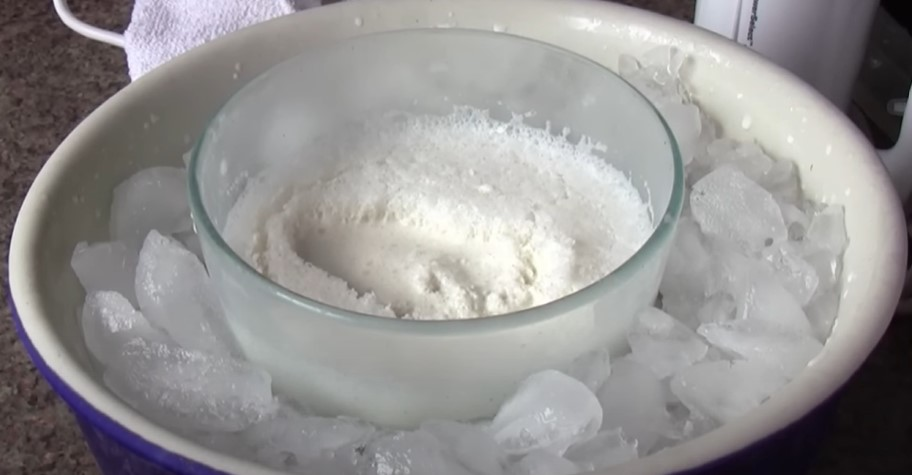
\includegraphics[width=0.35\linewidth]{../figs/VN12-Y24-PH-SYL-006P-1}
		\captionof{figure}{Kem lỏng nhanh chóng đông thành đá khi cho muối vào thau nước đá.}
	\end{center}
\begin{enumerate}[label=\alph*)]
	\item Kem lạnh đi do nhận nhiệt từ nước đá.
	\item Khi cân bằng nhiệt diễn ra, nếu trong đá có lẫn nước thì nhiệt độ của hỗn hợp nước và nước đá là $\SI{0}{\celsius}$.
	\item Nước muối thấm qua tô vào kem và làm tăng nhiệt độ đông đặc của kem (kem đông đặc ở nhiệt độ trên $\SI{0}{\celsius}$).
	\item Nhiệt độ đông đặc của nước trong thau sau khi cho muối vào bị giảm.
\end{enumerate}
\hideall{
\begin{enumerate}[label=\alph*)]
	\item Sai. Kem lạnh đi là do kem toả nhiệt cho thau đá.
	\item Đúng.
	\item Sai. Nước muối không thể thấm qua tô do sự liên kết của các phân tử chất rắn rất chặt chẽ. Ở điều kiện tiêu chuẩn, nhiệt độ đông đặc của nước là $\SI{0}{\celsius}$.
	\item Đúng. Nhiệt độ đông đặc của nước trong thau sau khi cho muối vào bị giảm là do sự phân li của các ion trong phân tử muối ăn làm ảnh hưởng đến liên kết hydrogen của các phân tử nước. Do đó, các phân tử nước khó liên kết lại với nhau thành thể rắn hơn
\end{enumerate}
}
\end{enumerate}
\section{Bài tập tự luận}
\begin{enumerate}[label=\bfseries Câu \arabic*:, leftmargin=1.7cm]
	\item \mkstar{2}\\
	Người ta bỏ một cục nước đá khối lượng $m_1=\SI{100}{\gram}$ vào một nhiệt lượng kế bằng đồng có khối lượng $m_2=\SI{125}{\gram}$, thì nhiệt độ của nhiệt lượng kế và nước đá là $t_1=\SI{-20}{\celsius}$. Tính nhiệt lượng cần thiết để làm tan được một nửa lượng nước đá trên. Cho nhiệt dung riêng của đồng là $c_2=\SI{380}{\joule/\kilogram\cdot\kelvin}$, của nước đá là $c_1=\SI{2100}{\joule/\kilogram\cdot\kelvin}$, nhiệt nóng chảy riêng của nước đá là $\SI{3.34E5}{\joule/\kilogram}$.
	\hideall{
Nhiệt lượng cần cung cấp cho nhiệt lượng kế để nước đá tan được 1 nửa:
$$Q=\left(m_1c_1+m_2c_2\right)\cdot\left(0-t_1\right)+\dfrac{m_1}{2}\lambda=\SI{21850}{\joule}.$$	
}

\item \mkstar{3}\\
Dẫn hơi nước ở $\SI{100}{\celsius}$ vào một bình nước đang có nhiệt độ $\SI{20}{\celsius}$ dưới áp suất bình thường.
\begin{enumerate}[label=\alph*)]
	\item Khối lượng nước trong bình tăng lên bao nhiêu lần khi nhiệt độ của nó đạt tới $\SI{100}{\celsius}$.
	\item Khi nhiệt độ của nước đạt tới $\SI{100}{\celsius}$, nếu tiếp tục dẫn hơi nước ở $\SI{100}{\celsius}$ vào bình thì có thể làm cho nước trong bình có thể sôi được không?
\end{enumerate}
Cho:
\begin{itemize}
	\item nhiệt dung riêng của nước $c=\SI{4200}{\joule/\left(\kilogram\cdot\kelvin\right)}$;
	\item nhiệt hoá hơi riêng của nước $L=\SI{2.3E6}{\joule/\kilogram}$.
\end{itemize}
\hideall{
\begin{enumerate}[label=\alph*)]
	\item Gọi $m$ là khối lượng hơi nước ngưng tụ và $M$ là khối lượng nước có sẵn trong bình.\\
	Khi có cân bằng nhiệt, tổng nhiệt lượng trao đổi trong hệ bằng 0:
	$$-mL+Mc\left(100-t_0\right)=0\Rightarrow m=0,146M.$$
	$$\Rightarrow \dfrac{m+M}{M}=1,146.$$
	\item Nước không thể sôi vì hệ đã đạt trạng thái cân bằng nhiệt ở $\SI{100}{\celsius}$ nên không thể nhận thêm nhiệt lượng để hoá thành hơi.
\end{enumerate}
}

\item \mkstar{3}\\
Người ta dẫn hơi nước ở $\SI{100}{\celsius}$ vào một nhiệt lượng kế chứa $\SI{100}{\gram}$ nước đá ở $\SI{0}{\celsius}$. Sau khi nước đá tan hết, khối lượng nước trong nhiệt lượng kế là bao nhiêu? Cho nhiệt nóng chảy riêng của nước đá là $\lambda=\SI{3.4E5}{\joule/\kilogram}$; nhiệt hoá hơi riêng của nước $L=\SI{2.26E6}{\joule/\kilogram}$; nhiệt dung riêng của nước $c=\SI{4200}{\joule/\left(\kilogram\cdot\kelvin\right)}$ và bỏ qua nhiệt dung của nhiệt lượng kế.
\hideall{
Gọi $m$ là khối lượng hơi nước ngưng tụ thành nước và $m_\text{đ}$ là khối lượng nước đá nóng chảy.\\
Khi có cân bằng nhiệt, tổng nhiệt lượng trao đổi của hệ bằng 0:
$$m_\text{đ}\lambda-mL+mc\left(0-100\right)=0\Rightarrow m=\SI{0.0127}{\kilogram}.$$
Lượng nước tăng thêm trong bình:
$$m_\text{n}=m_\text{đ}+m=\SI{112.7}{\gram}.$$
}

	\item \mkstar{3}\\
	Người ta đổ $\xsi{m_1}{\left(\kilogram\right)}$ nước ở nhiệt độ $t_1=\SI{60}{\celsius}$ vào $\xsi{m_2}{\left(\kilogram\right)}$ nước đá ở nhiệt độ $t_2=\SI{-5}{\celsius}$. Khi có cân bằng nhiệt, lượng nước thu được là $m=\SI{50}{\kilogram}$ có nhiệt độ $t=\SI{25}{\celsius}$. Xác định $m_1$ và $m_2$. Cho nhiệt dung riêng của nước và nước đá lần lượt là $c_1=\SI{4200}{\joule/\left(\kilogram\cdot\kelvin\right)}$, $c_2=\SI{2100}{\kilogram/\left(\kilogram\cdot\kelvin\right)}$, nhiệt nóng chảy riêng của nước đá $\lambda=\SI{3.4E5}{\joule/\kilogram}$.
	\hideall{
Ta có:
\begin{equation}
	\label{eq:6P-1}
	m_1+m_2=\SI{50}{\kilogram}
\end{equation}	
Khi cân bằng nhiệt xảy ra, tổng nhiệt lượng trao đổi trong hệ bằng 0:
$$m_1c_1\left(t_\text{cb}-t_1\right)+m_2c_2\left(0-t_2\right)+m_2\lambda+m_2c_1\left(t_\text{cb}-t_1\right)=0.$$
\begin{equation}
	\label{eq:6P-2}
	-147000m_1+455500m_2=0
\end{equation}
Từ (\ref{eq:6P-1}) và (\ref{eq:6P-2}), suy ra:
\begin{equation*}
	\begin{cases}
		m_1=\SI{37.8}{\kilogram}\\
		m_2=\SI{12.2}{\kilogram}
	\end{cases}
\end{equation*}
}

\item \mkstar{3}\\
Cho $\SI{100}{\gram}$ nước đá ở nhiệt độ $t_1=\SI{0}{\celsius}$ vào $\SI{300}{\gram}$ nước ở nhiệt độ $t_2=\SI{20}{\celsius}$. Hỏi nước đá có tan hết không? Nếu không, em hãy tính khối lượng nước đá còn lại.\\
Cho nhiệt nóng chảy riêng của nước đá là $\lambda=\SI{3.4E5}{\joule/\kilogram}$ và nhiệt dung riêng của nước là $c=\SI{4200}{\joule/\left(\kilogram\cdot\kelvin\right)}$.
\hideall{
Nhiệt lượng nước đá thu vào để nóng chảy hoàn toàn
$$Q_\text{thu}=m_\text{đ}\lambda=\SI{3.4E4}{\joule}.$$
Nhiệt lượng nước toả ra để giảm nhiệt độ từ $\SI{20}{\celsius}$ xuống $\SI{0}{\celsius}$:
$$Q_\text{toả}=m_\text{n}c\left(t_\text{n}-0\right)=\SI{2.52E4}{\joule}.$$
Vì $Q_\text{thu}>Q_\text{toả}$ nên nước đá không tan hết.\\
Gọi $m$ là khối lượng nước đá tan.\\
Do nước đá không tan hết nên nhiệt độ của hệ khi cân bằng nhiệt là $\SI{0}{\celsius}$.\\
Khối lượng nước đá tan:
$$m=\dfrac{Q_\text{toả}}{\lambda}\approx\SI{0.07412}{\kilogram}\approx\SI{74.12}{\gram}.$$
Vậy: khối lượng nước đá còn lại là xấp xỉ $\SI{25.88}{\gram}$.
}

\item \mkstar{3}\\
\begin{enumerate}[label=\alph*)]
	\item Tính nhiệt lượng do $\SI{500}{\gram}$ nước ở $\SI{30}{\celsius}$ toả ra khi nhiệt độ của nó hạ xuống $\SI{0}{\celsius}$.
	\item Để biến lượng nước trên thành nước đá, người ta bỏ vào nước trên một khối nước đá ở nhiệt độ $\SI{-10}{\celsius}$. Tính khối lượng nước đá tối thiểu cần dùng.
\end{enumerate}
Cho:
\begin{itemize}
	\item nhiệt dung riêng của nước $c_\text{n}=\SI{4200}{\joule/\left(\kilogram\cdot\kelvin\right)}$;
	\item nhiệt dung riêng của nước đá $c_\text{đ}=\SI{2000}{\joule/\left(\kilogram\cdot\kelvin\right)}$;
	\item nhiệt nóng chảy riêng của nước đá $\lambda=\SI{3.4E5}{\joule/\kilogram}$.
\end{itemize}
\hideall{
\begin{enumerate}[label=\alph*)]
	\item Nhiệt lượng do $\SI{500}{\gram}$ nước đá toả ra để hạ nhiệt độ từ $\SI{30}{\celsius}$ xuống $\SI{0}{\celsius}$:
	$$Q_1=m_\text{n}c_\text{n}\left(t_\text{n}-0\right)=\SI{63}{\kilo\joule}.$$
	\item Nhiệt lượng tối thiểu lượng nước trên cần toả ra để đông thành đá (nước đá ở $\SI{0}{\celsius}$):
	$$Q_\text{toả}=Q_1+m_\text{n}\lambda=\SI{233}{\kilo\joule}.$$
	Nhiệt lượng do đá ở $\SI{-10}{\celsius}$ thu vào để tăng nhiệt độ lên $\SI{0}{\celsius}$ bằng nhiệt lượng do nước toả ra, do đó khối lượng đá cần dùng:
	$$m_\text{đá}=\dfrac{Q_\text{toả}}{c_\text{đ}\left(0-t_\text{đ}\right)}=\SI{11.65}{\kilogram}.$$
\end{enumerate}
}

\item \mkstar{3}\\
Cho đồ thị biểu diễn sự thay đổi nhiệt độ của khối chất lỏng theo nhiệt lượng cung cấp có dạng như hình bên. Biết nhiệt dung riêng của chất lỏng đó là $c=\SI{2500}{\joule/\left(\kilogram\cdot\kelvin\right)}$. Xác định nhiệt hoá hơi riêng của chất lỏng trên.
\begin{center}
	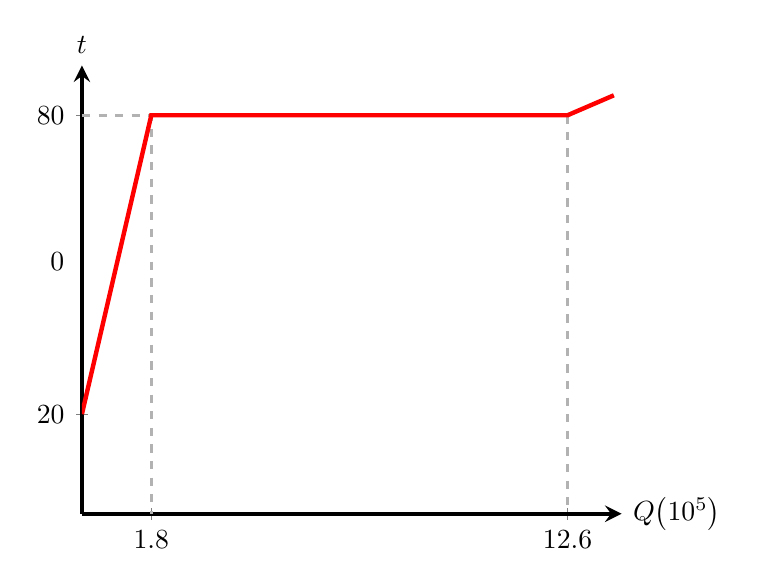
\begin{tikzpicture}  
		\begin{axis}[  ultra thick,
			xmin=0,  
			xmax=14,  
			xtick={1.8,12.6},
			ytick={20,80},
			minor x tick num=0,
			minor y tick num=0,
			ymin=0,  
			ymax=90, 
			samples=300,
			axis lines=center, 
			xlabel=$\xsi{Q}{\left(\xsi{10^5}{\joule}\right)}$, 		ylabel=$\xsi{t}{\celsius}$,
			every axis y label/.style={at=(current axis.above origin),anchor=south},  
			every axis x label/.style={at=(current axis.right of origin),anchor=west},  ]
			\draw [line width=1.0pt,dashed,gray!60!white] (axis cs: 0,80) --(axis cs: 1.8,80)--(axis cs: 1.8,0);
			\draw [line width=1.0pt,dashed,gray!60!white] (axis cs: 12.6,80)--(axis cs: 12.6,0);
			\draw [ultra thick, red] (axis cs: 0,20) --(axis cs: 1.8,80)--(axis cs: 12.6,80)--(axis cs: 13.8,84); 
			 
				\end{axis}
		\node[left] at (-0.1,3.2) {0};  
	\end{tikzpicture}
	
\end{center}
\hideall{
Nhiệt lượng chất lỏng thu vào để tăng nhiệt độ từ $\SI{20}{\celsius}$ lên $\SI{80}{\celsius}$:
$$Q_1=mc\left(t_2-t_1\right).$$
Nhiệt lượng chất lỏng thu vào để hoá hơi hoàn toàn ở nhiệt độ sôi:
$$Q_2-Q_1=mL.$$
Ta có:
$$\dfrac{Q_2-Q_1}{Q_1}=\dfrac{L}{c\Delta t}\Rightarrow L=\left(\dfrac{Q_2-Q_1}{Q_1}\right)c\Delta t=\left(\dfrac{\SI{12.6}{\joule}-\SI{1.8}{\joule}}{\SI{1.8}{\joule}}\right)\cdot\left[\SI{2500}{\joule/\left(\kilogram\cdot\kelvin\right)}\right]\cdot\left(\SI{80}{\celsius}-\SI{20}{\celsius}\right)=\SI{9E5}{\joule/\kilogram}.$$
}

\item \mkstar{4}\\
Thả 1 quả cầu bằng thép có khối lượng $m_1=\SI{2}{\kilogram}$ được nung tới nhiệt độ $\SI{600}{\celsius}$ vào một hỗn hợp nước và đá ở $\SI{0}{\celsius}$. Hỗn hợp có khối lượng tổng cộng là $m_2=\SI{2}{\kilogram}$.
\begin{enumerate}[label=\alph*)]
	\item Tính khối lượng nước đá có trong hỗn hợp. Biết nhiệt độ cuối cùng của hỗn hợp là $\SI{50}{\celsius}$.
	\item Thực ra, trong quá trình trên có một lớp nước tiếp xúc trực tiếp với quả cầu bị hoá thành hơi nên nhiệt độ cuối cùng của hỗn hợp chỉ là $\SI{48}{\celsius}$. Tính khối lượng nước đã hoá thành hơi.
\end{enumerate}
Cho:
\begin{itemize}
	\item nhiệt dung riêng của thép $c_1=\SI{460}{\joule/\left(\kilogram\cdot\kelvin\right)}$;
	\item nhiệt dung riêng của nước $c_2=\SI{4200}{\joule/\left(\kilogram\cdot\kelvin\right)}$;
	\item nhiệt nóng chảy riêng của nước đá $\lambda=\SI{3.4E5}{\joule/\kilogram}$;
	\item nhiệt hoá hơi riêng của nước $L=\SI{2.3E6}{\joule/\kilogram}$.
\end{itemize}
\hideall{
\begin{enumerate}[label=\alph*)]
	\item Gọi $m_\text{n}$ và $m_\text{đ}$ lần lượt là khối lượng nước và đá có trong hỗn hợp ban đầu.\\
	Khi cân bằng nhiệt, tổng nhiệt lượng trao đổi trong hệ bằng 0:
	$$m_\text{đ}\lambda+m_2c_2\left(t_\text{cb}-0\right)+m_1c_1\left(t_\text{cb}-t_1\right)=0$$
	$$\Leftrightarrow m_\text{đ}=\dfrac{m_1c_1\left(t_1-t_\text{cb}\right)-m_2c_2t_\text{cb}}{\lambda}=\SI{0.253}{\kilogram}.$$
	\item Phần nhiệt lượng bị mất mát đi khi chỉ đạt nhiệt độ cân bằng ở $\SI{48}{\celsius}$ thay vì $\SI{50}{\celsius}$ bằng nhiệt lượng $\xsi{m}{\left(\kilogram\right)}$ nước thu vào để tăng nhiệt độ từ $\SI{48}{\celsius}$ lên $\SI{100}{\celsius}$ và hoá hơi hoàn toàn:
	$$m_2c_2\left(50-48\right)=mc_2\left(100-48\right)+mL\Rightarrow m=\SI{6.67E-3}{\kilogram}=\SI{6.67}{\gram}.$$
\end{enumerate}
}

\end{enumerate}
